%%---------------------------------------------------------------------------%%
%% NSE Article
%% 2013: RQI+MGE
%%---------------------------------------------------------------------------%%

\documentclass[preprint,12pt]{elsarticle}
%\documentclass[12pt]{article}
\usepackage{amsmath}
\usepackage{amssymb,amsthm,graphicx}
\usepackage{epsfig}
\usepackage[mathcal]{euscript}
%\usepackage{citesort}
\usepackage{setspace}
%\usepackage{tmadd,tmath}
\usepackage{color}
\usepackage{array}
%\usepackage{c++}
%\usepackage{times, mathptm}
\usepackage{subfigure}
%\usepackage{dsfont}

\usepackage{times}
\renewcommand{\ttdefault}{cmtt}

\usepackage{fancyhdr} % used to put page number in header instead of footer

% The float package HAS to load before hyperref
\usepackage{float} % for psuedocode formatting
\usepackage{xspace}
\usepackage{mathrsfs}
\usepackage[pdftex]{hyperref}

\usepackage{graphicx}
\graphicspath{{images/}}

%%---------------------------------------------------------------------------%%

%\setlength{\textfloatsep}{8pt plus 1pt minus 1pt}
%\setlength{\abovedisplayskip}{4pt plus 1pt minus 1pt}
%\setlength{\belowdisplayskip}{4pt plus 1pt minus 1pt}
%\addtolength{\oddsidemargin}{-0.5in}
%\addtolength{\textwidth}{1.0in}
%\addtolength{\textheight}{0.5in}

\setlength{\textwidth}{6.5in}
\setlength{\oddsidemargin}{0.0in}
\setlength{\evensidemargin}{0.0in}
\setlength{\textheight}{9.0in}
\setlength{\topmargin}{0.0in}
\setlength{\headheight}{0.0in}
\setlength{\headsep}{0.0in}
\setlength{\footskip}{0.5in}

\renewcommand{\thefootnote}{\fnsymbol{footnote}}
\renewcommand{\thetable}{\Roman{table}}

%%---------------------------------------------------------------------------%%

\newcommand{\email}[1]{$\langle$#1@pitt.edu$\rangle$}

\DeclareMathOperator{\diag}{diag}
\DeclareMathOperator{\low}{lower}
\DeclareMathOperator{\upp}{upper}

\newcommand{\Sn}{\ensuremath{S_N}}
\newcommand{\Macro}{\ensuremath{\Sigma}}

\newcommand{\vOmega}{\ensuremath{\hat{\Omega}}}
\newcommand{\Ye}[2]{\ensuremath{Y^e_{#1}(\vOmega_#2)}}
\newcommand{\Yo}[2]{\ensuremath{Y^o_{#1}(\vOmega_#2)}}

\newcommand{\ve}[1]{\ensuremath{\mathbf{#1}}}

\newcommand{\sigg}[1]{\ensuremath{\sigma^{gg'}_{\text{s}\,#1}}}
\newcommand{\psig}{\ensuremath{\psi^g}}

\newcommand{\even}{\ensuremath{\phi^g}}
\newcommand{\odd}{\ensuremath{\vartheta^g}}

\newcommand{\evenp}{\ensuremath{\phi^{g'}}}
\newcommand{\oddp}{\ensuremath{\vartheta^{g'}}}

\newcommand{\apsi}[1]{\ensuremath{\psi^{\dagger\,#1}}}
\newcommand{\aeven}[1]{\ensuremath{\phi^{\dagger\,#1}}}
\newcommand{\aodd}[1]{\ensuremath{\vartheta^{\dagger\,#1}}}
\newcommand{\asigg}[1]{\ensuremath{\sigma^{g'g}_{\text{s}\,#1}}}

\newcommand{\aPsi}[1]{\ensuremath{\Psi^{\dagger\,#1}}}
\newcommand{\aPhi}[1]{\ensuremath{\Phi^{\dagger\,#1}}}

\newcommand{\epsi}{\ensuremath{\epsilon}}
\newcommand{\ephi}{\ensuremath{\varepsilon}}

\newcommand{\psie}{\ensuremath{\psi_{\epsi}}}
\newcommand{\phie}{\ensuremath{\phi_{\ephi}}}

\newcommand{\Psie}{\ensuremath{\Psi_{\epsi}}}
\newcommand{\Phie}{\ensuremath{\Phi_{\ephi}}}

\newcommand{\apsie}[1]{\ensuremath{\psi^{\dagger\,#1}_{\epsi}}}
\newcommand{\aphie}[1]{\ensuremath{\phi^{\dagger\,#1}_{\ephi}}}

\newcommand{\aPsie}[1]{\ensuremath{\Psi^{\dagger\,#1}_{\epsi}}}
\newcommand{\aPhie}[1]{\ensuremath{\Phi^{\dagger\,#1}_{\ephi}}}

\newcommand{\avg}[1]{\ensuremath{\langle#1\rangle}}

\newcommand{\osig}{\ensuremath{\overline{\sigma}}}
\newcommand{\osigs}{\ensuremath{\overline{\sigma_{\text{s}}}}}

%%---------------------------------------------------------------------------%%

\begin{document}

\setcounter{page}{2}
  
%%---------------------------------------------------------------------------%%

\begin{center}

  {\large \bf Title}
  
  \vspace{0.3in}
  
  R.N.\ Slaybaugh, M.\ Ramirez-Zweiger, Tara Pandya, Steven Hamilton, and T.M.\ Evans
  
\end{center}

\doublespacing

\vspace{0.3in}

\begin{abstract}

  Abstract

\end{abstract}

\newpage

%%---------------------------------------------------------------------------%%

\section{Introduction}
\label{sec:intro}
The steady-state Boltzmann equation for neutron transport covers six dimensions of phase space. Typical deterministic transport problems today are three-dimensional, have up to thousands $\times$ thousands $\times$ thousands of mesh points, use up to $\sim$150 energy groups, include accurate expansions of scattering terms, and are solved over many angular directions. The next generation of challenging problems are even more highly refined. High-fidelity, coupled, multiphysics calculations are the new ``grand challenge'' problems for reactor analysis, requiring that the finely-resolved neutron flux be calculated quickly and accurately.

Very large computers, such as Titan \cite{Titan2013}, are available to perform such high-fidelity calculations. Historical solution methods are not able to take full advantage of new computer architectures, or they have convergence properties that limit their usefulness for difficult problems. The goal of this research is to accelerate transport calculations with methods that use new computers fully and effectively, facilitating the design of better nuclear systems. 

Three complimentary methods have been implemented in the code Denovo \cite{Evans2010} that accomplish this goal: a multigroup block (MG) Krylov solver, a Rayleigh Quotient Iteration (RQI) eigenvalue solver, and a multigrid in energy (MGE) preconditioner. Each individual method has been described before (see \cite{Slaybaugh2012}, \cite{Slaybaugh2013}), but this is the first time they have been demonstrated to work together effectively.

The driving concept of this research is to use RQI for solving the $k$-eigenvalue problem in 3-D neutron transport. This objective was not tractable with the tools originally available in Denovo. The multigroup Krylov solver and multigrid-in-energy preconditioner were developed to facilitate RQI, though both of these tools are also useful on their own. 

The multigroup Krylov solver was designed to improve convergence when compared to Gauss Seidel (GS) and to dramatically increase the number cores Denovo can use. Instead of sequentially solving each group with some inner iteration method and then using GS for outer iterations to converge the upscattering, the MG Krylov solver treats a block of groups (either all groups or just upscattering groups) at once such that the inner-outer iteration structure is removed. This results in faster convergence for most problem types. In addition, the block Krylov solver allows energy groups to be solved simultaneously because the multigroup-sized matrix vector multiply can be divided up in energy and parallelized. This extends the number of cores that can be used efficiently by Denovo from tens of thousands to hundreds of thousands. 

A multigrid in energy preconditioner was added to Denovo to reduce iteration count for all problem types, and to address convergence issues associated with RQI. The  preconditioner conducts a multigrid method in the energy dimension. A set of energy grids with increasingly coarse energy group structures are created. This is implemented in a way that easily and efficiently takes advantage of the new energy decomposition. The multigrid algorithm is applied within each energy set such that the energy groups are only restricted and prolonged between groups on that set. Sets do not communicate with one another in the preconditioner, so the scaling in energy is very good. 

Theory indicates that RQI should converge in fewer iterations than traditional eigenvalue solvers like power iteration, particularly for problems that are challenging for those solvers. However, the use of RQI would not be practical without the MG Krylov solver and the MGE preconditioner. The implementation of RQI results in a set of equations that is mathematically equivalent to having upscattering in every group, so the scattering matrix becomes energy-block dense. Handling energy-block dense systems when there are more than a few energy groups is not tractable with GS as the multigroup solver. It is only the MG Krylov solver that makes RQI reasonable to use when there are many energy groups. In addition, the MGE preconditioner is needed to mitigate the slow convergence associated with Krylov methods when trying to solve the ill-conditioned systems created by RQI. 

The remainder of this paper presents information about why these methods are complementary as well as results demonstrating that they are. Section \ref{sec:background} discusses each of the new methods in the context of commonly-used methods. Section \ref{sec:pastwork} gives an overview of relevant past work. New results from using the three new methods together are shown in Section \ref{sec:results}, and concluding remarks are made in Section \ref{sec:conclusions}.

%%---------------------------------------------------------------------------%%
%%---------------------------------------------------------------------------%%
%%---------------------------------------------------------------------------%%
\section{Background}
\label{sec:background}
% The eigenvalue form of the steady state Boltzmann transport equation is
% \begin{align}
%    [\hat{\Omega} \cdot \nabla + \Macro(\vec{r}, E)] &\psi(\vec{r}, \hat{\Omega}, E)  = \frac{\chi(E)}{k} \int_0^{\infty} dE' \:\nu \Macro_{f}(\vec{r}, E') \int_{4\pi} d\hat{\Omega'} \:\psi(\vec{r}, \hat{\Omega'}, E') \nonumber \\
%    &+ \int_0^{\infty} dE' \int_{4\pi} d\hat{\Omega'} \:\Macro_{s}(\vec{r}, E' \to E, \hat{\Omega'} \cdot \hat{\Omega}) \psi(\vec{r}, \hat{\Omega'}, E') \:,
% \label{eq:neutron transport}
% \end{align}
% %
% \noindent where the quantities are at location $\vec{r}$, at energy E, and are traveling in direction $\hat{\Omega}$. The angular neutron flux in neutrons per unit length squared per steradian is $\psi(\vec{r}, \hat{\Omega}, E)$, which expresses the location of the neutrons in phase space; $\Macro_{x}$ is the cross section that represents the likelihood of interaction $x$ (here $s$ is for scattering, $f$ is for fission, and no subscript indicates all interactions) in units of inverse length. Here $\chi(E)$ is the spectrum specifying the energy distribution of neutrons born from fission, $k$ is the asymptotic ratio of the number of neutrons in one
% generation to the number in the next, and $\nu$ is the average number of neutrons released per fission. In the fixed source case, the fisission term can be replaced by an external source, $q_{ex}$ \cite{Lewis1993}. 
% 
% To numerically solve Equation~\eqref{eq:neutron transport} it is discretized in space, angle, and energy. This work uses the multigroup energy approximation, the scattering term is expanded in Legendre polynomials ($P_l$), and discrete ordinates (\Sn) are used to treat direction of neutron travel. There are many spatial differencing methods available, the discussion of which is beyond the scope of this document as the proposed work is not dependent upon the spatial discretization employed \cite{Evans2009d}. To ensure the new methods apply to the most general cases, it will be assumed that the matrices resulting from discretization are not necessarily symmetric. 
%
%After all of the discretizations are performed, t
The multigroup $S_N$ equations can be written in operator form as
%
\begin{alignat}{2}
  \ve{L}\psi &= \ve{MS}\phi + q \:, \qquad &\text{(fixed source)} \label{eq:fxdsource} \\
  \ve{L}\psi &= \ve{MS}\phi + \frac{1}{k}\ve{M}\chi f^{T}\phi \:. \qquad &\text{(eigenvalue)} \label{eq:eigenvalue}
\end{alignat}
%
Here $\ve{L}$ is the first-order linear differential transport operator; $\ve{M}$ is the moment-to-discrete operator that projects the angular flux moments, $\phi$, onto discrete angles; $\ve{S}$ is the scattering matrix; $q$ is a source term; $f$ contains the fission source, $\nu \Macro_{f}$; $\chi$ is the energy distribution with which neutrons are born out of fission; and $k$ is the asymptotic ratio of the number of neutrons in one generation to the number in the next. The angular flux moments are related to the angular flux, $\phi$ through the discrete-to-moment operator: $\phi = \mathbf{D} \psi \:$. Using this relationship, Equations \eqref{eq:fxdsource} and \eqref{eq:eigenvalue} can be rearranged such that they are a function of only $\phi$. The formulation is aided by defining $\ve{T} = \ve{DL}^{-1}$ and $\ve{F} = \chi f^{T}$ \cite{Evans2011}:
%
\begin{alignat}{2}
  (\ve{I} - \ve{TMS})\phi &= q \:, \qquad &\text{(fixed source)} \label{eq:OperatorFxdForm} \\
  (\ve{I} - \ve{TMS})\phi &= \frac{1}{k} \ve{TMF} \phi \:. &\text{(eigenvalue)} \label{eq:OperatorEvalForm}
\end{alignat}

Once the matrices are multiplied together, a series of single ``within-group'' equations that are each only a function of space and angle result. If the groups are coupled together by neutrons scattering from a low energy group to a higher energy group, then iterative ``multigroup'' solves over the coupled portion of the energy range may be required. If the eigenvalue is desired, an additional ``eigenvalue'' solve is needed where $k$ is the dominant eigenvalue and $\phi$ is the corresponding eigenvector \cite{Evans2009}. 

%%---------------------------------------------------------------------------%%
%%---------------------------------------------------------------------------%%
\subsection{Block Krylov Solver}
\label{sec:blockkrylov}
Traditionally, the multigroup solve has been done with Gauss Seidel. GS is iterative in energy. A space-angle solve using a within-group solver, such as source iteration or a Krylov method, is performed for each energy group in series. The groups are solved from $g=0$, the highest energy, to $g=G$, the lowest. For a group $g$ and an energy iteration index $j$ this is \cite{Evans2010}
%
\begin{equation}
  \bigl( \ve{I} - \ve{TMS}_{gg} \bigr) \phi^{j+1}_{g} = \ve{TM} \bigl( \sum_{g'=0}^{g-1}\ve{S}_{gg'}\phi^{j+1}_{g'} + \sum_{g'=g+1}^{G} \ve{S}_{gg'}\phi^{j}_{g'}  + q_{g} \bigr)  \:.
 \label{eq:up-GS}
\end{equation}

The first term on the right includes downscattering contributions from higher energies, and the second term represents upscattering contributions from lower energy groups that have not yet been converged for this energy iteration. Groups that only contain downscattering are simply solved once since the second term on the right is zero. Groups with upscattering, however, must be iterated until they converge. Convergence of GS is governed by the spectral radius of the system, so the method can be very slow when upscattering has a large influence on the solution \cite{Adams2002}. GS is fundamentally serial in energy because of how the group-to-group coupling is treated. 

The multigroup (MG) Krylov solver removes the traditional ``within-group'' / ``multigroup'' iteration structure by combining the space-angle and energy iterations to make one space-angle-energy iteration level. This allows the energy groups to be decomposed such that they can be solved in parallel. The space-angle-energy iterations are much like the within-group space-angle iterations, except that the iteration is over a block of groups instead of just one group. There are two energy decomposition strategies: all groups and upscatter groups only. When only the upscatter groups are decomposed into sets, the downscatter groups are replicated and solved using GS while the upscatter groups are solved with a Krylov solver. For full partitioning, all groups are decomposed into sets and only the Krylov solver is used. 

The multigroup Krylov method applied to the upscattering block is shown here, where $\ve{S}_{\text{up\_block}}$ contains the upscattering groups and $\ve{S}_{\text{up\_source}}$ has the downscattering-only groups:
%
\begin{equation}
  \underbrace{(\ve{I} - \ve{TMS}_{\text{up\_block}})}_{\tilde{\ve{A}}}\phi_{\text{up\_block}}^{n+1} = \ve{TM}(\ve{S}_{\text{up\_source}}\phi_{\text{up\_source}}^{n+1} + q) \:.
  \label{eq:MGkrylov}
\end{equation}
%
Trilinos \cite{1089021} provides Denovo's Krylov solver, with a choice of either GMRES($m$) or BiCGSTAB \cite{Evans2010}. The Krylov solver is given an operator that implements the action of $\ve{\tilde{A}}$, or the matrix-vector multiply and sweep. In the MG Krylov solver, $\ve{\tilde{A}}$ is applied to an iteration vector, $v$, containing the entire upscattering block instead of just one group.%:
%
% \begin{enumerate}
%   \item matrix-vector multiply: $y = \ve{M}\ve{S}_{\text{up\_block}} v$,
%   \item sweep: $z = \ve{T} y$,
%   \item return: $v \leftarrow v - z$.
% \end{enumerate}

To implement the energy parallelization, the problem is divided into energy sets, with groups distributed evenly among sets. After each set performs its part of the matrix-vector multiply, a global reduce-plus-scatter is the only required inter-set communication. Since each set uses the entire spatial mesh with the same spatial decomposition, the established performance of spatial scaling does not change. The space-angle decomposition in Denovo comes from the KBA wavefront algorithm \cite{Baker1998}. %Evans et al.\ \cite{Evans2009d} showed scaling in space is limited to about 20,000 cores with a 500 million cell spatial mesh. 

The added energy decomposition offers the ability to further decompose a problem, even if the performance limit of spatial decomposition has been reached. The total number of cores is equal to the number of computational domains, that is, the product of the number of energy sets and the number of spatial blocks. For 20,000 spatial blocks and 10 energy sets, which is a reasonable decomposition, 200,000 cores will be used. See Ref.\ \cite{Evans2011} for more details. 

The solver has been shown to successfully scale to hundreds of thousands of cores. For example, a fixed-source test scaled from 69,102 cores to 190,080 cores with 98\% efficiency \cite{Slaybaugh2011}. Upscatter partitioning has been shown to initially perform better than full partitioning, but does not scale well over many energy sets \cite{Davidson2013}. An added benefit of this solver is that Krylov methods generally converge more quickly than GS for problems with upscattering \cite{Trefethen1997}.
% Note: Davidson 2014 isn't in the bib file...where is this citation?

%%---------------------------------------------------------------------------%%
%%---------------------------------------------------------------------------%%
\subsection{Eigenvalue Solvers}
\label{sec:eigenvalue}
Denovo has three eigenvalue solver choices, Power Iteration, Rayleigh Quotient Iteration, and Arnoldi. 

\subsubsection{Power Iteration}
A common way to solve $k$-eigenvalue problems is with Power Iteration (PI). This method is attractive because it only requires matrix-vector products and two vectors of storage space. 
%
\begin{align}
  \ve{A}\phi &= k\phi \:, \label{eq:EnergyDepEval} \\
  \qquad \text{where}  \qquad \ve{A} &= (\ve{I} - \ve{TMS})^{-1} \ve{TMF} \:, \nonumber \\
  \phi^{i+1} = \frac{1}{k^i}\ve{A}\phi^{i} &\:; \qquad 
  k^{i+1} = k^i \frac{f^T \phi^{i+1}}{f^T \phi^i} \:.
  \label{eq:PowerIteration}
\end{align} 
%
PI uses the form of the problem seen in Eq. \eqref{eq:EnergyDepEval} and then iterates as shown in Eq.\ \eqref{eq:PowerIteration}, where $i$ is the iteration index. This converts the generalized form of the eigenvalue problem seen in Eq.\ \eqref{eq:OperatorEvalForm} to the ordinary form. In the generalized form, the eigenvector-value pair is $(\phi, \frac{1}{k})$, and in the ordinary form it is $(\phi, k)$. 
In legacy applications, the eigenvector is often the fission source rather than the flux moments \cite{Evans2011}, \cite{Lewis1993}.
Inside of PI, the application of $\ve{A}$ to $\phi$ requires the solution of a multigroup problem that looks like a fixed source problem,
\begin{equation}
  (\ve{I} - \ve{TMS})y^{i} = \ve{TMF}\phi^{i} \:. \label{eq:EvalDepFxdSource}
\end{equation}

PI's convergence can be very slow for problems of interest. For an $n \times n$ matrix $\ve{A}$, an eigenvalue-vector pair satisfies $\ve{A}x_{i} = \lambda_{i}x_{i}$ for $i = 1,...,n$. Let $\sigma(\ve{A}) \equiv \{\lambda \in \mathbb{C} : $\\$ rank(\ve{A} - \lambda \ve{I}) \le n\}$ be the spectrum of $\ve{A}$ and the eigenvalues be ordered as $|\lambda_{1}| > |\lambda_{2}| \ge \dots $\\$\ge |\lambda_{n}| \ge 0$. The error from PI is reduced in each iteration by a factor of $\ve{A}$'s dominance ratio, $\frac{\lambda_{2}}{\lambda_{1}}$. PI will converge slowly for loosely coupled systems because $\lambda_{2}$ is close to $\lambda_{1}$ \cite{Trefethen1997}. 

\subsubsection{Rayleigh Quotient Iteration}
Shifted inverse iteration (SII) typically converges more quickly than PI. SII capitalizes on the fact that for some shift $\mu$, $(\ve{A} - \mu \ve{I})$ will have the same eigenvectors as $\ve{A}$. If $\mu \notin \sigma(\ve{A})$, then $(\ve{A} - \mu \ve{I})$ is invertible and $\sigma([\ve{A} - \mu \ve{I}]^{-1}) = \{1/(\lambda - \mu):\lambda \in \sigma(\ve{A})\}$. Eigenvalues of $\ve{A}$ that are near the shift will be transformed to extremal eigenvalues that are well separated from the others. The shifted and inverted matrix is used in a power iteration-type scheme. Given a good shift, $\mu \approx \lambda_1$, SII usually converges more quickly than PI, especially for loosely coupled systems \cite{Trefethen1997}, \cite{Allen2002}.

% Wielandt's method is a flavor of SII that has been used widely in the neutron transport community, though it was originally developed in 1944 in an unrelated context \cite{Zinzani2008}, \cite{Itagaki1996}, \cite{Itagaki2002}. In the transport equation formulation, Wielandt's method changes the eigenvalue problem to $(\ve{I} - \ve{TM}(\ve{S} +\gamma_e \ve{F}))\phi = \delta \gamma \ve{TMF} \phi$, where $\gamma_e$ is the current estimate for the dominant eigenvalue, $\gamma_1 = \frac{1}{k}$, and $\delta \gamma = \gamma_1 - \gamma_e$. The power method is applied to this, giving \cite{Nakamura1977}
% %
% \begin{equation}
% \phi^{i+1} = \delta \gamma^{i}(\ve{I} - \ve{TM}(\ve{S} + \gamma_e \ve{F}))^{-1}\ve{TMF}\phi^{i} \:. \label{eq:Wielandt}
% \end{equation}

Rayleigh Quotient Iteration is a shifted inverse iteration method %similar to Wielandt's method, but it 
that uses an optimal shift: the Rayleigh quotient (RQ). For a generalized eigenvalue problem $\beta \ve{A}x = \alpha \ve{B}x$, the RQ is
%
\begin{equation}
  \rho = \frac{y^{T} \ve{A} x}{y^{T} \ve{B} x} \:.
  \label{eq:RQ}
\end{equation}
%
If $x$ and $y$ are right and left eigenvectors corresponding to $\alpha$ and $\beta$, respectively, then $\alpha = y^{T} \ve{A} x$ and $\beta =  y^{T} \ve{B} x$. In this case, $\rho = \gamma$, where $\gamma = \frac{\alpha}{\beta}$ \cite{Stewart2001}. The RQ provides the minimum residual for the eigenvalue problem in the least squares sense, where equivalence holds only when $\tau = \rho$ and $x \ne 0$:
%
\begin{equation}
  ||(\ve{A} - \tau\ve{B})x||^{2} \ge ||\ve{A}x||^{2} - ||\rho\ve{B}x||^{2} \:.
\end{equation}
%
The Rayleigh quotient is thus an optimal guess for an eigenvalue given a vector close to the corresponding eigenvector \cite{Parlett1974}. 

The idea of RQI is to use the RQ as the shift in SII and update it with the new eigenvector estimate at every iteration $i$:
%
\begin{equation}
  \mu_i = \gamma_{i-1} - \rho_i \:.
  \label{eq:Shift}
\end{equation} 
%
RQI has better convergence properties than SII since the RQ is an optimal guess for the eigenvalue of interest. For more details on the Rayleigh quotient and RQI in general, refer to Ref.\ \cite{Parlett1974}.

RQI has been implemented in Denovo, as detailed in Ref.\ \cite{Slaybaugh2012}, by subtracting $\rho \ve{TMF}$ from both sides of Eq.\ \eqref{eq:OperatorEvalForm}. This gives the following shifted system, where $\gamma \equiv \frac{1}{k}$:
%
\begin{align}
  (\ve{I} - \ve{TM}\ve{\tilde{S}})\phi &=( \gamma - \rho) \ve{TMF} \phi  \:, 
  \label{eq:OperatorShiftedEval} \\
  \text{ where } \ve{\tilde{S}} &\equiv \ve{S} + \rho\ve{F}  \nonumber \:.
\end{align}
%
The new matrix, $\ve{\tilde{S}}$, is energy-block dense since the fission matrix is dense and looks like one big upscattering block. Traditional solution methods for the fixed source part of the equation do not handle dense scattering matrices well. This has hampered the implementation of SII in multi-group, 3-D codes because solving many groups that have upper-triangular scattering entries can be time-prohibitive. 

The RQI method added to Denovo uses the MG Krylov solver, which is designed to handle dense scattering matrices effectively, to overcome the use of a dense $\ve{\tilde{S}}$. In addition, RQI can be decomposed in energy and take advantage of the scaling properties of the multigroup solver. Using RQI in combination with a Krylov method, however, raises some concerns about whether or not it can converge. 

%A method's behavior can be affected by characteristics of the mathematical problem as well as by characterisitics of the algorithm. Conditioning is one way to express the perturbation behavior of the mathematical problem. An ill-conditioned problem is one in which some small perturbation of $x$ leads to a large change in $f(x)$. A large condition number corresponds to an ill-conditioned problem, and vice versa. 

On initial consideration it would seem shifted inverse methods might not work well when the shift is very good because the matrix becomes so ill-conditioned. Peters and Wilkinson \cite{Peters1979}, however, proved that ill-conditioning is not a fundamental problem for inverse iteration methods. Trefethen and Bau \cite{Trefethen1997} assert that this is the case as long as the fixed source portion is solved with a backwards stable algorithm. 

Paige et al.\ \cite{Paige2006} demonstrated that GMRES is backwards stable when finding $x$ in $\ve{A}x = b$ for a ``sufficiently nonsingular $\ve{A}$'', and define associated criteria. For ill-conditioned systems, then, Krylov methods may not be backwards stable and will tend to converge very slowly. Many researchers have found that Krylov methods must be preconditioned to be able to get good results in practice \cite{Benzi2002}, \cite{Saad1986}, \cite{Trefethen1997} , \cite{Paige2006}. The past work section below demonstrates that RQI does need preconditioning for convergence in problems of interest.

\subsubsection{Arnoldi}
Denovo has also implemented an Arnoldi Krylov subspace solver available for solving eigenvalue problems \cite{Davidson2013}. 
It can take either an energy-dependent or energy-independent form. Consider the energy dependent eigenvalue equation 
\begin{equation}
\begin{split}
\mathbf{A}\phi &= k \phi, \\
\mathbf{A} &= (\mathbf{I} - \mathbf{TMS})^{-1}\mathbf{TMF}
\end{split}
\end{equation}
We then perform a matrix-vector multiply/sweep and fixed source solve.
\begin{equation}
z^{(h)} = \mathbf{TMF}\nu^{(h)}.
\end{equation}
\begin{equation}
(\mathbf{I} - \mathbf{TMS})y^{(h)} = z^{(h)}.
\end{equation}
The energy independent case takes the form
\begin{equation}
\begin{split}
\mathbf{A}\Gamma &= k\Gamma, \\
\mathbf{A} &= \mathbf{f}^T(\mathbf{I - TMS})^{-1}\mathbf{TM\chi}.
\end{split}
\end{equation}
Like in the energy-dependent case, a matrix-vector multiply/sweep and a fixed-source solve are performed with an additional matrix-vector multiply after.
\begin{equation}
z^{(h)} = \mathbf{TM\chi}\nu^{(h)}
\end{equation}
\begin{equation}
(\mathbf{I} - \mathbf{TMS})x^{(h)} = z^{(h)}
\end{equation}
\begin{equation}
y^{(h)} = \mathbf{f}^Tx^{(h)}
\end{equation}
Note that the vectors in the energy-dependent subspace span all of the energy groups, whereas the energy-independent approach requires each vector to span just one, using less memory. However, when the flux moments as well as the eigenvalue are desired, the energy-independent approach requires a final fixed source solve, potentially losing its memory advantage. The fixed-source solve is given by
\begin{equation}
(\mathbf{I} - \mathbf{TMS})\phi = \frac{1}{k}\mathbf{TM\chi\Gamma},
\end{equation}
Where k is the eigenvalue and $\Gamma$ is the eigenvector. It is not immediately evident which approach will be best suited to a given problem, so both approaches, energy-dependent and energy-independent, are considered. In the two cases convergence behavior is nearly identical given that their nonzero eigenvalues are the same. Like RQI, the Arnoldi solver can be parallelized over energy by using energy sets enabled by the MG Krylov solver.


\subsection{Multigrid in Energy Preconditioner}
\label{sec:precond}
%For many kinds of problems, the total number of multigroup iterations required to adequately converge the transport equation is large. To reduce iteration count, a preconditioner can be applied to transform the system of interest into another equivalent system that has more favorable properties and is easier to solve. 
Preconditioning is important for increasing the robustness of Krylov methods and decreasing Krylov iteration count. This is particularly true for the multigroup Krylov solver. This solver can create large Krylov subspaces because it forms the subspaces with multiple-group-sized vectors. As a result, any reduction in iteration count will have a significant benefit in terms of memory and cost per iteration. 
 
Right preconditioning leaves the right hand side of the equation unaffected and does not change the norm of the residual, which is used for convergence testing in most iterative methods. A right preconditioner that does multigrid in the energy dimension and is designed to work with the MG Krylov solver was implemented in Denovo \cite{Slaybaugh2013}. To understand why multigrid in energy makes sense for neutron transport, some highlights about these methods are discussed here (derived from Ref.\ \cite{Briggs2000}). 

The error in $x_i$, the $i$th guess for $\ve{A}x_i=b_i$, can be written as a combination of Fourier modes. Each Fourier mode has a frequency, and the frequencies can range from low-frequency (smooth) to high-frequency (oscillatory). Iterative methods, also referred to as smoothers or relaxers, remove high-frequency error components quickly, but take many iterations to remove the low-frequency ones. 

The idea of multigrid methods is to take advantage of the smoothing effects of iterative methods by making smooth errors look oscillatory and thus easier to remove. Errors that are low-frequency on a fine grid can be mapped onto a coarser grid where they are high-frequency. A relaxer is applied on the coarser grid to remove the now oscillatory error components. The remaining error is mapped to a still coarser grid and smoothed again. The problem is restricted to coarser and coarser grids until it is on a grid that is coarse enough to directly invert the equations.

Next, the coarsest result is prolonged back to the next-finer grid and used to correct the solution there. A few relaxations are done on this finer grid. The errors are prolonged back up the grid structure, continuously correcting on finer grids, until the finest grid is reached. This entire process is called a V-cycle. %Multigrid methods are differentiated by how many times the V-cycle is done and how many grids are used. The optimal combination of grids and cycles may depend on problem type. The addition of more grids and cycles will reduce error, but at an added cost.
 
Thus, multigrid methods remove the low-frequency error modes that require many Krylov iterations. The preconditioner was designed to take advantage of the energy decomposition used by the MG Krylov method. Each energy set does work only on its own grids and does not need to communicate with other energy sets. This is a communication savings compared to using grids in space or angle. An additional benefit is the simplicity of energy grids. Energy is one-dimensional, which allows for simpler coarsening and refinement than spatial or angular grids.

To implement multigrid in energy as a right preconditioner in Denovo, the problem is broken into two steps shown below. Here $\ve{G}^{-1}$ represents the appication of the preconditioner, and $y$ is defined as $\ve{G}\phi$; recall that $\ve{A} = \ve{I} - \ve{TMS}$.  
%
\begin{enumerate}
  \item With a Krylov method solve 
    \begin{equation}
      \ve{AG}^{-1}y = b \:, \label{eq:PrecondKrylov} 
    \end{equation}
  \item after finding $y$, calculate 
    \begin{equation}
      \phi = \ve{G}^{-1}y \:. \label{eq:PrecondPhi}
    \end{equation}
\end{enumerate}

%Note: it is possible to implement the preconditioner using the shifted operator (used in RQI) rather than the unshifted operator. It is expected that the unshifted operator will be a much better choice for the obvious reasons of stability. However, we implemented the option to use either for investigation purposes. 

In this preconditioner the grids are in energy, where the energy group structure is coarsened so that each lower grid has fewer groups. The finest grid is the input energy structure, and the coarsest grid has one or a few groups. Each level has half as many groups as the previous level, rounded up if applicable. If there are $G+1$ groups on the fine grid there will be either $\frac{G+1}{2}$ or $\frac{G+2}{2}$ groups on the coarse grid. This is conceptually straightforward because the energy groups can be combined (restricted) and separated (prolonged) linearly. For details on the implementation of the preconditioner consult Ref. \cite{Slaybaugh2013}
%
%The implemented restriction operator is a simple averaging scheme. Neighboring fine data are averaged together to make coarse data. To prolong from a coarse to a fine grid, the points that line up between the grids are mapped directly. To fill in the intermediate points on the fine grid, the adjacent coarse values are averaged. There are other restriction and prolongation operators that are more rigorous and would preserve more accuracy when transferring between grids than those implemented. However, the implemented methods were found to be sufficient in practice.

The user chooses the number of V-cycles done for each preconditioner application. One V-cycle proceeds from the finest grid to the coarsest grid and back to the finest. Each additional V-cycle should remove more error, but has a computational cost. The depth of the V-cycle can also be specified by the user. The default behavior is determined by the number of groups, such that the grids will be coarsened until there is only one energy group. The number of grids needed is $\text{floor}\bigl( \log_{2}(G-1) \bigr) + 2$ \cite{BinaryTree2012}.% given by \cite{BinaryTree2012}
%\begin{equation}
%  num\_grids = \text{floor}\bigl( \log_{2}(G-1) \bigr) + 2 \:.
%  \label{eq:NumGrids}
%\end{equation}

When using multiple energy sets, cross-set communication is prohibited by having each set do its own ``mini'' V-cycle. Each set restricts, prolongs, and relaxes on only its own groups. In the case of an unequal number of groups per set, all sets are forced to have the same grid depth to enforce energy load balancing between sets. Thus, each set restricts to one or two groups, giving approximately $num\_sets$ total groups across all sets at the coarsest level. The number of grids needed is determined by the set with the minimum number of groups, since it will be the first to reach a grid with one group:%. This modifies Equation~\eqref{eq:NumGrids} to be
\begin{align}
  num\_g_{min} &= \text{floor}\bigl(\frac{num\_groups}{num\_sets}\bigr) \:, \\
  num\_grids &= \text{floor}\bigl( \log_{2}(num\_g_{min}) \bigr) + 2 \:.
  \label{eq:multisetGrids}
\end{align}

Some number of relaxations are performed on each level while traversing down and up the grids in a V-cycle. Performing more relaxations per grid should remove more error, but has a computational cost. The implemented relaxation method is weighted Richardson Iteration. When applied to the transport equation, this is
%
\begin{equation}
  \phi^{m} = \bigr(\ve{I} + \omega(\ve{TMS} - \ve{I})\bigl)\phi^{m-1} + \omega b^{m-1} \:,
  \label{eq:relax}
 \end{equation}
%
where $\omega$ is a constant selected by the user that defaults to 1 and $m$ is iteration index. 

An important principle is that the preconditioner is only attempting to approximately invert $\ve{A}$. It is therefore reasonable to use a less accurate angular discretization in the preconditioner than the rest of the code. For example, the whole problem may be solved at $S_{10}$, but the preconditioner could use $S_{2}$. The user can specify an angular quadrature set to use in the preconditioner that is different from the angular quadrature set used in the rest of the problem; the default is to use the same quadrature in both. At this time, this option has only been implemented for vacuum boundary conditions. 

%%---------------------------------------------------------------------------%%
%%---------------------------------------------------------------------------%%
%%---------------------------------------------------------------------------%%
\section{Past Work}
\label{sec:pastwork}
This section is a summary of results using RQI with preconditioning \cite{Slaybaugh2012} and the MGE Preconditioner with fixed source problems or PI \cite{Slaybaugh2013}. The purpose of this section is to highlight the capabilities that have been demonstrated and point out the short-comings that can be overcome by using the MG Krylov solver, RQI eigenvalue solver, and MGE preconditioner together. In the following discussion, reducing the Krylov iteration count is the primary measure of success--with reduced time as the second consideration. A discussion of this choice is given at the beginning of the Section \ref{sec:results}, Results.

\subsection{Unpreconditioned RQI}
The goal of the RQI studies that have been published was to find out it if RQI useful without preconditioning. We solved two small eigenvalue test problems, one with vacuum boundaries and one with reflecting, that had small dominance ratios. We found that RQI got the correct answer and converged in fewer iterations than power iteration. However, an itermediately-sized problem did not work so well. Each multigroup solve, except the first, used the maximum number of Krylov multigroup iterations per eigenvalue iteration. This means the eigenvector did not converge after the first iteration. The value of $k$ oscillated between 0.3966 and 0.3967 (the correct value was 0.4) until the calculation was manually terminated. In two more realistic calculations, the 2D and 3D C5G7 MOX Benchmark problems (described in subsections \ref{subsec:2dc5g7} and \ref{subsec:3dc5g7}, respectively), RQI did not converge the eigenvector nor find an eigenvalue close to the correct one. 

These more challenging problems showed that, as expected, the Krylov solver often cannot converge the eigenvector with the ill-conditioned systems created by RQI. When the Krylov iterations do not converge, the flux estimate is not good. Without an adequate approximation to the eigenvector, the RQ is no longer a valid approximation to the eigenvalue, and therefore the eigenvalue problem does not converge. 

The small problems showed that RQI can require fewer Krylov iterations than PI, and has the potential to be beneficial if the multigroup iterations are converged. If the MG Krylov solver is preconditioned so that the eigenvector converges, RQI may be able to find the correct eigenvalue more efficiently than PI for cases of interest. This leads to the question: what preconditioner should we choose?

Iterative methods reduce oscillatory error modes effectively, but not smooth error modes. The smooth error can prevent iterative methods from converging. This behavior is characterized by rapid error reduction in the first several iterations followed by very little error reduction. Such a trend was observed is tests where RQI failed. Multigrid methods selectively remove smoother error components and are therefore ideal for accelerating this type of problem. Thus, a multigrid preconditioner should work very well with RQI. 

\subsection{MGE Preconditioner}
Much of the previously published work for the MGE preconditioner focused on choosing all of the options that control the preconditioner. The preconditioning parameters are the Richardson iteration weight, $w_{k}$, the number of V-cycles per preconditioner application, and the number of relaxations per level. The syntax used throughout this work will be that $w\#$ is the weight, $r\#$ is the number of relaxations per level, and $v\#$ is the number of V-cycles, e.g.\ $w1r1v1$ is one relaxation per level, one V-cycle, and a weight of one. Using more preconditioning means using larger values of $w$ and/or $r$ and/or $v$. 

Some initial tests provided a basis for chosing preconditioning parameters. The results showed that increasing $r$ and/or $v$ decreased Krylov iteration count, as expected. They also indicated that using a small amount of weight can be beneficial, but a large amount is not. As a result, the parameters are set to default to $w1r2v2$. Other issues investigated were using a different quadrature set inside the preconditioner than in the rest of the problem, strong scaling, and changing the depth of the V-cycle. 

Tests showed that using a reduced angle set inside the preconditioner is very valuable. For example, using $S_2$ inside MGE for an iron-graphite test solved with $S_8$ reduced the solve time by 73\% compared to using $S_8$ in the preconditioner.

Another important area of investigation was how the preconditioner faired when using multiple energy sets because MGE was built to take advantage of multiple energy sets. The problems solved scaled about 40\% more efficiently with MGE preconditioning than without it. The main reason for the preconditioner’s good scaling is that as the number of sets increases, each application of the preconditioner becomes less costly. 

The total preconditioning cost goes down because the V-cycle becomes shallower. When 27 groups are used with one set, six grids are created. When 27 groups are used with 10 sets, two grids are created for each set. With fewer grids each application of the preconditioner performs fewer total relaxations, and is therefore less time intensive. The number of GMRES iterations did not change with the number of sets in the preconditioned cases. This means convergence improvement from the preconditioner did not come from the depth of the V-cycle, at least not for the problems tested.

The results of the multiple energy set study prompted an investigation of controlling V-cycle depth explicitly. The results from several tests confirm the multiple energy set study findings: using only a few grids is better than using many. The optimal number of grids will be problem dependent, but a default grid depth of two was recommended.

All of these tests inform the best way to use the MGE preconditioner, but do not determine whether and when it is useful. To begin investigating this question, two eigenvalue problems were solved with preconditioned and unpreconditioned PI. The first problem was the 3D C5G7 MOX Benchmark problem. In this case the use of MGE significantly reduced Krylov iteration count, but increased the overall runtime. A full PWR problem (described in subsection \ref{subsec:PWR}) exhibited similar behavior: fewer iterations in more time. 

These results suggest that the MGE preconditioner was a failed experiment after all. However, the two eigenvalue problems solved were not particularly challenging for PI, meaning they may not have needed preconditioning to begin with. More importantly, the mathematical properties of the MGE preconditioner suggest it would benefit the RQI solver. Thus, the work published so far has not settled the question of whether MGE is a useful preconditioner for at least some problems. 

%%---------------------------------------------------------------------------%%
\section{Results}
\label{sec:results}
%The collection of observations in the past work section led to the questions (1) Will preconditioning with MGE facilitate the use of RQI? and (2) Will the combination of RQI, MGE, and the block Krylov solver be advantagous for at least some problems? This section covers a series of problems designed to answer these two questions. 

%The goal of using this system of solvers is to improve convergence behavior of the multigroup Krylov solves integrated over eigenvalue solves. The best metric for measuring this is the total number of multigroup Krylov iterations used in a calculation because it is the most consistent and fair measure. The number of eigenvalue iterations is also compared for the eigenvalue tests. This is a point of interest rather than a measure of goal attainment. The total number of Krylov iterations is the best proxy for convergence behavior as it encompasses the work that is done within each eigenvalue iteration.  

%Timing comparisons should be considered heuristically unless otherwise specified. In cases where the calculations were done on a single core, the machine was not dedicated to these calculations and times could vary if the same calculations were repeated. Some problems use an optimized version of the code and others use a debug version. These should give the same iteration count, but not necessarily the same relative times between problems. Further, little effort has been made to optimize the preconditioner for speed. Once the multigrid in energy preconditioner has been optimized for efficiency, the preconditioned times should decrease. How much improvement can be gained is a matter for future study. 

%Unless otherwise noted, all test problems used a step characteristic spatial solver, level-symmetric angular quadrature, and the grid depth was determined using the default approach. %, Equation~\eqref{eq:NumGrids} or Equation~\eqref{eq:multisetGrids}. 
%The Krylov solver was GMRES, which is set to limit the number of multigroup iterations to 1,000 if the problem does not converge earlier. The convergence tolerances are noted for each problem. The tolerance for the multigroup solve is the convergence tolerance used by GMRES in Trilinos \cite{1089021}. The eigenvalue tolerance is used by PI to determine if the eigenvalue has converged. In Denovo, PI also checks the L2-norm and the infinity-norm of the difference in the fission source between iterations. The default L2-norm tolerance is 1.0 and infinity-norm tolerance is 0.01.

%\subsection{Initial Investigation}
%A variety of small problems were solved to verify code functionality, ensure that total Krylov count is reduced by the addition of MGE, verify MGE parameter choice when used in combination with RQI, and confirm that the preconditioner should \emph{not} use the shifted version of the operator.
%
%The first test problem set was that initially solved with unpreconditioned RQI, which included a vacuum and a reflecting boundary case. The addition of MGE with the unshifted preconditioner to the vacuum test always resulted in the correct solution in fewer Krylov iterations than the unpreconditioned case. The number of RQ iterations was not affected by the preconditioning. The reflecting case with the unshifted operator reduced both total Krylov iteration count and eigenvalue iteration count, except for cases in which $r1v1$ was used with a weight of 1.2 or higher. Larger $r/v$ combinations did not have difficulty with a weight of 1.2. These cases confirmed that the solvers could work together, that the correct solution is obtained as long as the problem converges, that Krylov iteration count is reduced when RQI is used with MGE, and the parameter guidance previously established is still valid. 
%
%The tests were repeated with the shifted operator inside of MGE. In the vacuum case, fewer Krylov iterations were needed than with the unshifted operator. However, with the smallest set of $r/v/w$ the correct solution was not always found. When the shifted operator was used with the reflecting case, the problem often did not converge. These tests confirmed that the problems associated with shifting the operator persist when used inside of Richardson iteration, and that the unshifted version should be used to ensure stability. 
%
% \subsubsection{Intermediate problem}
% RQI kinda choked on this without preconditioning, but behaved really really poorly with preconditioning. This was the one with negative fluxes and complete crazy behavior that we never explained. Worked fine with MGE+PI. Worked worse with BiCGSTAB instead of GMRES. 
% 
% \begin{table}[!h]
% \caption{Infinite Medium Eigenvalue Problem, Preconditioning Results with Rayleigh Quotient Iteration}
% \begin{center}
% \begin{tabular}{| c | c | c | c | l | c | c | c | c |}
% \hline
% $w$ & $r$ & $v$ & $k$ & Krylov & RQI & Max Rel Diff & RMS Err & Rel Time$^{+}$ \\[0.5ex]
% \hline
% 0    & 0 & 0 & 0.3970 & 39,025              & 40$^{*}$  & n/a & n/a & 211.03 \\%$5.43 \times 10^{4}$ \\
% 1    & 1 & 1 & 0.3982 & 3,014$^{\dag}$ & 4 & $1.67 \times 10^{-1}$ & $3.32 \times 10^{-2}$ & 103.56 \\%$2.66 \times 10^{4}$ \\
% 1    & 3 & 1 & 0.3983 & 50                     & 3 & 0.0 & 0.0 & 40.19 \\ %$1.03 \times 10^{4}$ \\
% 1    & 4 & 1 & 0.3983 & 44$^{\dag}$      & 3 & 0.0 & 0.0 & 4.51 \\ %$1.16 \times 10^{3}$ \\
% 1    & 2 & 2 & 0.3983 & 44$^{\dag}$      & 3 & 0.0 & 0.0 & 1.11 \\ %$2.86 \times 10^{2}$ \\
% 1    & 4 & 4 & 0.4001 & 16                     & 3 & $1.67 \times 10^{-1}$ & $3.21 \times 10^{-2}$ & 7.73 \\ %$1.99 \times 10^{3}$ \\
% 1    & 5 & 4 & 0.4001 & 14$^{\dag}$     & 3 & $1.67 \times 10^{-1}$ & $3.21 \times 10^{-2}$ & 8.81 \\ %$2.27 \times 10^{2}$ \\
% 1.4 & 5 & 4 & -0.4711 & 12$^{\dag}$    & 2 & $1.67 \times 10^{-1}$ & $3.21 \times 10^{-2}$ & 6.77 \\ %$1.74 \times 10^{3}$ \\
% 1    & 5 & 5 & -0.4575 & 7$^{\dag}$      & 2 & $3.43 \times 10^{-6}$ & $3.67 \times 10^{-5}$ & 6.13 \\ %$1.58 \times 10^{3}$ \\
% \hline
% 1.1 & 4 & 1 & 0.3983 & 43$^{\dag}$      & 3 & 0.0 & 0.0 & 4.51 \\ %$1.16 \times 10^{3}$ \\
% 1.1 & 1 & 4 & 0.3983 & 43$^{\dag}$      & 3 & 0.0 & 0.0 & 5.24 \\ %$1.35 \times 10^{3}$ \\
% 1.1 & 2 & 2 & 0.3983 & 43$^{\dag}$      & 3 & 0.0 & 0.0 & 4.57 \\ %$1.18 \times 10^{3}$ \\
% \hline
% 0.7 & 1 & 1 & 0.3999 & 3,001$^{\dag}$ & 4 & 1.0 & $3.72 \times 10^{-1}$ & 87.34 \\ %$2.25 \times 10^{4}$ \\
% 0.7 & 3 & 1 & 0.4001 & 87$^{\dag}$      & 5 & 0.0 & 0.0 & 7.60 \\ %$1.95 \times 10^{3}$ \\
% 0.7 & 3 & 3 & 0.4001 & 47$^{\dag}$      & 5 & 0.0 & 0.0 & 11.34 \\ %$2.92 \times 10^{3}$ \\
% 0.4 & 3 & 1 & 0.4001 & 1,052$^{\dag}$ & 4 & $1.18 \times 10^{-5}$ & $8.43 \times 10^{-8}$      & 67.57 \\ %$1.74 \times 10^{4}$ \\
% \hline 
% \end{tabular}\\
% $^{+}$compared to unpreconditioned PI, $2.57 \times 10^{2}$ seconds\\
% $^{*}$terminated manually\\
% $^{\dag}$negative flux
% \end{center}
% \label{table:impi RQI}
% \end{table}
% %
% The preconditioned results are shown in Table~\ref{table:impi RQI}. In the table ``Max Rel Diff'' is the maximum over all cells and all groups of the relative difference between the reference flux and the absolute value of the computed flux, $\max[ (\phi_{ref} - \vert\phi_{calc}\vert) / \phi_{ref}]$. ``RMS Err'' is the root mean squared (rms) relative error, $\sqrt{ \sum_{1}^{N}(rel\_err)^{2} / N}$. As a reminder, the total and upscattering tolerances were $1 \times 10^{-4}$, and the $k$ tolerance was $1 \times 10^{-5}$. Recall that if the Krylov iteration count is in the thousands it means the eigenvector did not converge in every iteration. The ``Rel Time'' column is the ratio of the found time to the unpreconditioned PI time of $2.57 \times 10^{-2}$ seconds.
% 
% ** Should we leave this out?\\
% ** Should we try to understand this better?\\
% ** Is it unethical to leave out this data?\\
%
%\subsubsection{2D C5G7}
%\label{subsec:2dc5g7}
%After the baseline was established, MGE was applied to the 2-D C5G7 benchmark using both PI and RQI with the goals of seeing if preconditioned RQI could converge the flux and $k$, to investigate the effect of preconditioning in both RQI and PI, and to see whether the lessons learned about preconditioning parameters still hold in a real problem. The calculation used 16 cores on the small orthanc cluster at Oak Ridge: 4 $x$-blocks, 4 $y$-blocks, 1 $z$-block and 1 energy set. The total and upscattering tolerances were $1 \times 10^{-3}$, with a $k$ tolerance of $1 \times 10^{-5}$. An optimized version of Denovo was used.  
%
%A weight variation study was done with power iteration first. The results using $r1v1$ are plotted as Krylov Iterations vs.\ Weight, and Time in seconds vs.\ Weight in Figure~\ref{fig:2-Dc5g7PI}. All calculated $k$s were within the uncertainty of the benchmark and so are not reported. All preconditioned cases needed 31 power iterations while the unpreconditioned case took 32.
%%
%\begin{figure}[!ht]
%    \begin{center}
%      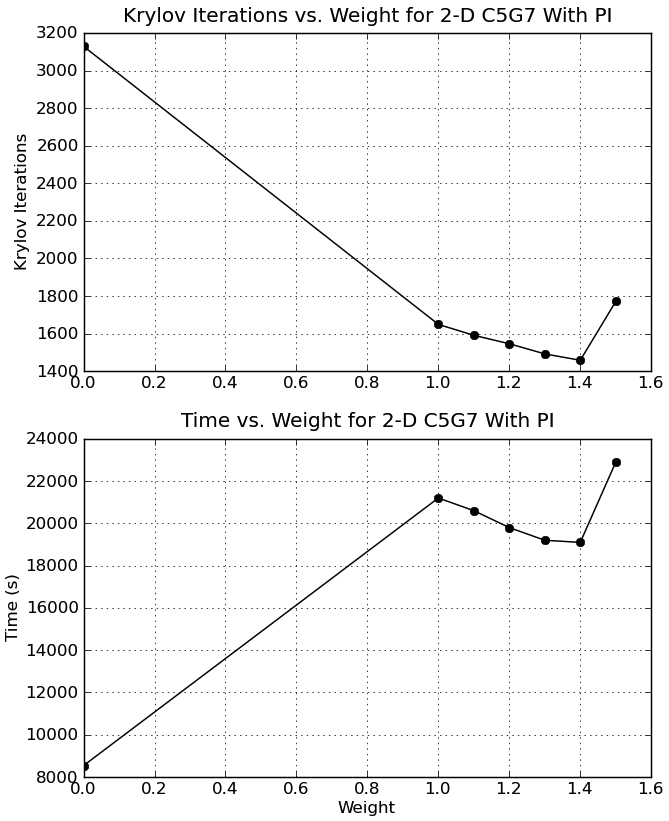
\includegraphics [width=0.7\textwidth, height=0.7\textheight] {2Dc5g7PI}
%   \end{center}
%   \caption{2-D C5G7 Benchmark, Preconditioner Weight Variation with Power Iteration}
%   \label{fig:2-Dc5g7PI}
%\end{figure}
%
%This study shows the preconditioner is very effective at reducing the number of Krylov iterations used by PI. The unpreconditioned case, corresponding to a weight of 0 on the plot, took 3,129 MG Krylov iterations. As the weight was increased from 1 to 1.4, the number of Krylov iterations and the time to solution both decreased. With $w1.4$, 1,458 MG Krylovs were taken. The time and iteration count both went back up with a weight of 1.5. When the weight was increased beyond 1.5 none of the multigroup iterations converged, and the problem was terminated manually after several power iterations. 
%
%Two other calculations with a higher level of preconditioning were also done. When the parameters were $w1.4r2v2$ the number of Krylov iterations were reduced to 438 and the calculation took $1.77 \times 10^{4}$ seconds, both lower than all the cases using $r1v1$. For $w1r3v3$, 253 Krylov iterations and $2.28 \times 10^{4}$ seconds were required. This had the smallest number of Krylov iterations, but a slightly longer time than all the calculations except $w1.5r1v1$.	
%
%The results from the RQI study are in Table~\ref{table:2-D c5g7 rqi}. In all cases, except the unpreconditioned one, $k$ was within the uncertainty of the benchmark value. The ``$<$ 1,000?'' column indicates whether or not the multigroup iterations converged during the RQI process. If the value is ``no,'' the eigenvector only converged during the first iteration. A number indicates the last eigenvalue iteration for which the Krylov method took less than 1,000 iterations. All subsequent iterations required the full 1,000. A ``yes'' means all of the Krylov iterations converged. The relative time is the ratio of the case of interest to the unpreconditioned PI time of $8.54 \times 10^{3}$ seconds.
%%
%\begin{table}[!h]
%\caption{2-D C5G7 Benchmark, Convergence Study with Rayleigh Quotient Iteration}
%\begin{center}
%\begin{tabular}{| c | c | c | l | c | c | c |}
%\hline
%Weight & Relaxations & V-cycles & Krylov & RQI & $<$ 1,000? & Rel Time$^{\dag}$\\[0.5ex]
%\hline
%0    & 0 & 0 & 119,006 & 120$^{*}$ & no & 10.98 \\%$9.38 \times 10^{4}$ \\
%1    & 1 & 1 & 16,007   & 17            & no & 23.65 \\ %$2.02 \times 10^{5}$ \\
%1.2 & 1 & 1 & 40,008   & 41$^{*}$   & no & 13.00 \\ %$2.06 \times 10^{5}$ \\
%1    & 3 & 1 & n/a         & n/a$^{*}$  & 7   & n/a \\
%1    & 2 & 2 & 11,158   & 19            & alternated & 46.72 \\ %$3.99 \times 10^{5}$ \\
%1    & 3 & 2 & 3,320     & 19            & 14 &19.23 \\ % $1.64 \times 10^{5}$ \\
%\hline
%1    & 3 & 3 & 299        & 19            & yes & 3.01 \\ %$2.57 \times 10^{4}$ \\
%1.1 & 3 & 3 & 281        & 19            & yes & 2.80 \\ %$2.40 \times 10^{4}$ \\
%1.3 & 3 & 3 & 254        & 19            & yes & 2.57 \\ %$2.19 \times 10^{4}$ \\
%1.5 & 3 & 3 & n/a         & n/a$^{*}$ & no & n/a \\
%\hline 
%\end{tabular} \\
%$^{\dag}$compared to unpreconditioned PI, $8.54 \times 10^{3}$ seconds\\
%$^{*}$terminated manually
%\end{center}
%\label{table:2-D c5g7 rqi}
%\end{table}
%
%These results show a few important things. Most significantly, with enough preconditioning the multigroup iterations within RQI can be converged and the correct eigenpair can be found. This was true even when the eigenvector did not converge inside each eigen iteration (though these cases were significantly more time consuming). Further, as the preconditioning increased the eigenvector came closer to converging for all iterations. For the first three $w\#r3v3$ cases, all of the Krylov iterations converged. This test case was the first to demonstrate that the preconditioner can get RQI to converge. Finally, when the Krylov iterations did converge, increasing the weight decreased iteration count and wall time for small weights but too much weight prevented the calculation from converging.
%%Additionally, it seems that preconditioning held RQI on track enough to get the right eigenvalue when the eigenvector did not quite converge. As was hypothesized for the unpreconditioned infinite medium test, it may be that the eigenvector was close enough to correct that a good approximation to the eigenvalue could still be made from it, even though the vector itself did not converge. 
%
%Only the $w1r3v3$ calculation overlaped between RQI and PI. PI took fewer Krylov iterations, 253 compared to 299, and less time, $2.28 \times 10^{4}$ compared to $2.57 \times 10^{4}$ seconds. For this test preconditioned RQI did not perform as well as preconditioned PI, though the times and iteration counts were close to one another. 
%
%From the standpoint of comparing eigenvalue solution methods, it is worth noting that RQI required 19 eigenvalue iterations while PI required 31. Thus, when given eigenvectors that have been converged to the same tolerance, RQI needed fewer eigenvalue iterations than PI. For this benchmark, though, preconditioned RQI took more Krylov iterations within each multigroup solve to get the eigenvector to that tolerance, so RQI was not better than PI in terms of total Krylov count.
%%
%The RQI problem was also tried with BiCGSTAB as the Krylov solver for an unpreconditioned case and a $w1r3v3$ case. Every multigroup iteration went to the 1,000 iteration limit and the problem was terminated manually after several RQ iterations.
%
%\subsection{Problems of Interest}
%While the first few small problems were useful for initial investigation, we are really interested in solving much larger, more complex problems. 
%
%\subsubsection{3D C5G7}
%\label{subsec:3dc5g7}
%The preconditioner using both PI and RQI was applied to the 3-D C5G7 benchmark with an optimized version of Denovo. The goals of this study were essentially the same as the 2-D study, except that this problem is larger, and the first to approach a real ``grand challenge'' type of calculation. The medium-sized oic cluster at Oak Ridge was used, and each problem was given 720 cores with 40 $x$-blocks, 18 $y$-blocks, and 5 $z$-blocks. The total and upscattering tolerances were $1 \times 10^{-4}$, with a $k$ tolerance of $1 \times 10^{-5}$ unless otherwise indicated. The wall time limit was 12 hours. Note that on the oic machine, if a calculation exceeds wall time there is no way to get any of the results from the scratch space. 
%
%The power iteration results were reported in \cite{Slaybaugh2013}, so we only add the RQI results here, which are shown in Table~\ref{table:3-D c5g7 rqi}.
%% and are in Table~\ref{table:3-D c5g7}. The relative time is compared to unpreconditioned PI, $4.46 \times 10^{3}$ seconds. The unpreconditioned power iteration calculation computed a $k$ that was not within the uncertainty bounds of the reported benchmark; it was low by about 0.011. All preconditioned PI and RQI tests computed a $k$ that was within the Denovo $k$ tolerance of the unpreconditioned PI result so they are not reported here. Subsequent to these calculations it was determined that using a more accurate quadrature gives the correct $k$. 
% 
% \begin{table}[!h]
% \caption{3-D C5G7 Benchmark, Preconditioning Parameter Scoping with Power Iteration}
% \begin{center}
% \begin{tabular}{| c | c | c | c | l | c |}
% \hline
% Weight & Relaxations & V-cycles & Krylov & PI & Rel Time$^{\dag}$ \\[0.5ex]
% \hline
% 0    & 0 & 0 & 1,224 & 32 & 1.00 \\ %$4.46 \times 10^{3}$ \\
% 1    & 1 & 1 & 708    & 32 & 5.90 \\ %$2.12 \times 10^{4}$ \\
% 1.2 & 1 & 2 & 448    & 32 & 5.33 \\ %$2.38 \times 10^{4}$ \\
% 1.2 & 2 & 1 & 448    & 32 & 5.37 \\ %$2.39 \times 10^{4}$ \\
% 1.3 & 2 & 2 & 288    & 32 & 6.37 \\ %$2.84 \times 10^{4}$ \\
% 1    & 3 & 3 & 126    & 14$^{*}$  & 9.05 \\ %$4.04 \times 10^{4}$ \\
% 1.5 & 3 & 3 & 192    & 32 & 8.36 \\ %$3.73 \times 10^{4}$ \\
% 1    & 4 & 4 & n/a     & n/a          & exceeded wall time \\
% 1    & 4 & 4 & n/a     & n/a$^{*}$ & exceeded wall time \\
% 1.5 & 5 & 5 & n/a     & n/a          & exceeded wall time \\
% \hline 
% \end{tabular}\\
% $^{\dag}$compared to unpreconditioned PI, $4.46 \times 10^{3}$ seconds\\
% $^{*}$tol and upscatter tol = $1 \times 10^{-5}$, $k$ tol = $1 \times 10^{-3}$
% \end{center}
% \label{table:3-D c5g7}
% \end{table}
% 
% The 3-D benchmark study shows the preconditioner with PI can reduce the number of required Krylov iterations substantially for challenging problems. The number of eigenvalue iterations for a given tolerance set were never changed by preconditioning. 
% 
% The effect of preconditioning parameters was consistent with what was observed in other test problems. However, using large values for $r$ and $v$ made the calculation take too long to get results. On the oic machine, if a calculation exceeds wall time there is no way to get any of the results from the scratch space. Therefore, no conclusions can be drawn from this problem about the effect of substantial preconditioning when using power iteration for a real, 3-D problem. 
%
%The RQI results are in Table~\ref{table:3-D c5g7 rqi}. 
%The relative time is compared to unpreconditioned PI, $4.46 \times 10^{3}$ seconds. Many cases did not finish in time to report results. What is likely happening when the problems with lower parameter values run out of time is that the eigenvector is not converging. As was seen before, the calculations take a long time when every eigenvalue iteration uses 1,000 Krylov iterations. Unfortunately, there is no way to confirm this or find out if the eigenvalue is close to correct since the output cannot be obtained. 
%%
%\begin{table}[!h]
%\caption{3-D C5G7 Benchmark, Preconditioning Parameter Scoping with Rayleigh Quotient Iteration}
%\begin{center}
%\begin{tabular}{| c | c | c | c | l | c |}
%\hline
%Weight & Relaxations & V-cycles & Krylov & RQI & Rel Time$^{+}$ \\[0.5ex]
%\hline
%0    & 0 & 0 & n/a     & n/a          & exceeded wall time \\
%1    & 1 & 1 & n/a     & n/a          & exceeded wall time \\
%1.5 & 1 & 1 & n/a     & n/a          & exceeded wall time \\
%1.2 & 2 & 1 & n/a     & n/a          & exceeded wall time \\
%1.3 & 2 & 2 & 302    & 19           & 5.20 \\ %$2.32 \times 10^{4}$ \\
%1    & 3 & 3 & 103    & 9$^{*}$    & 6.67 \\ %$3.02 \times 10^{4}$ \\
%1    & 3 & 3 & 164    & 15$^{\dag}$ & 7.59 \\ %$3.38 \times 10^{4}$ \\
%1.5 & 3 & 3 & 187    & 19           & 7.26 \\ %$3.24 \times 10^{4}$ \\
%1    & 4 & 4 & n/a     & n/a          & exceeded wall time \\
%1    & 4 & 4 & 74     & 9$^{*}$    & 5.13 \\ %$2.29 \times 10^{4}$ \\
%1.5 & 5 & 5 & n/a     & n/a          & exceeded wall time \\
%\hline 
%\end{tabular}\\
%$^{+}$compared to unpreconditioned PI, $4.46 \times 10^{3}$ seconds\\
%$^{*}$tol and upscatter tol = $1 \times 10^{-5}$, $k$ tol = $1 \times 10^{-3}$\\
%$^{\dag}$tol and upscatter tol = $1 \times 10^{-4}$, $k$ tol = $5 \times 10^{-5}$
%\end{center}
%\label{table:3-D c5g7 rqi}
%\end{table}  
%
%With an intermediate amount of preconditioning, RQI converged and performed better than the analogous PI cases. There are three cases where both problems finish and the same tolerances were used: $w1.3r2v2$, $w1r3v3$, $w1.5r3v3$. These results are shown together in Table~\ref{table:PI RQI} for ease of comparison. This table displays time instead of relative time since the comparison is between two cases rather than across all cases. In all three, the RQI calculations took less time and fewer eigenvalue iterations than PI. In the second two, they also took fewer Krylov iterations. RQI even finished in time to get results from the $w1r4v4$ calculation when PI did not. 
%%
%\begin{table}[!h]
%\caption{3-D C5G7 Benchmark, Rayleigh Quotient Iteration and Power Iteration Comparison}
%\begin{center}
%\begin{tabular}{| c | c | c | c | c | c | c |}
%\hline
%Sovler & Weight & Relaxations & V-cycles & Krylov & Eigenvalue & Time (s) \\[0.5ex]
%\hline
%RQI & 1.3 & 2 & 2 & 302    & 19           & $2.32 \times 10^{4}$ \\
%PI    & 1.3 & 2 & 2 & 288    & 32           & $2.84 \times 10^{4}$ \\
%\hline
%RQI & 1    & 3 & 3 & 103    & 9$^{*}$   & $3.02 \times 10^{4}$ \\
%PI    & 1    & 3 & 3 & 126    & 14$^{*}$ & $4.04 \times 10^{4}$ \\
%\hline
%RQI & 1.5 & 3 & 3 & 187    & 19           & $3.24 \times 10^{4}$ \\
%PI    & 1.5 & 3 & 3 & 192    & 32           & $3.73 \times 10^{4}$ \\
%\hline 
%\end{tabular}\\
%$^{*}$tol and upscatter tol = $1 \times 10^{-5}$, $k$ tol = $1 \times 10^{-3}$
%\end{center}
%\label{table:PI RQI}
%\end{table}  
%
%The 3-D benchmark problem shows that for at least some problems, preconditioned RQI converges more quickly in all senses than preconditioned PI. It is pertinent that this is true is the most interesting problem shown so far. It seems, however, that RQI can only be useful if it is preconditioned enough to get the eigenvector to converge. 
%%
%%These results continue to confirm that a small amount of weight works well for real problems. Increasing $r$ and $v$ decrease iteration count, but at what can be a high time penalty. An intermediate amount of preconditioning will likely provide the best balance of reduced iteration count for the time invested once the preconditioner is optimized. 
%%
%%** Could do more of these with better w,r,v choices to have more overlap between RQI and POI; use reduced angle set; not much grid depth to reduce, but could try anyway **
%
%\subsection{PWR 900 new results}
%\label{subsec:PWR}
%Most cases: tolerance = 1e-3, L2 tolerance = 1e-3, k tolerance = 1e-3. 578 x 578 x 700 cells (233,858,800 cells), 112 x 112 x 10 partitions (12,544 blocks). $S_{12}$, P0, 44 groups. 1.73 trillion unknowns. k0 = 1. Depth of V-cycle = 2, \Sn  in MGE = $S_2$
%%
%\begin{table}[!h]
%\caption{PWR-900 Comparison of PI and RQI with and without preconditioning on 11 energy sets}
%\label{tab:PWR all}
%  \begin{center}
%    \begin{tabular}{| c | c | c | c | c | c | c |}
%      \hline
%      Method & Precond & N Eigen & N Krylov & k & time (m) \\\hline
%      %%
%      RQI & none   & info &     &                     & \\
%      RQI & w1r1v1 & 3   & 45   & 1.252 $\pm$ 1.13e-2 & 120$^*$ \\
%      RQI & w1r2v2 & 5   & 70   & 1.268 $\pm$ 9.75e-4 & 54.8 \\
%      PI  & none   & 149 & 5602 & 1.276 $\pm$ 4.34e-6 & 612.2 \\
%      PI  & w1r1v1 & info &     &                     & \\
%      PI  & w1r2v2 & 86  & 946  & 1.275 $\pm$ 1.43e-5 & 720$^*$ \\
%      \hline
%      PI  & none   & 24  & 901  & 1.272 $\pm$ 1.01e-4 & 92.1$^\dagger$ \\
%      PI  & w1r1v1 & info &     &                     & \#$^\dagger$\\
%      PI  & w1r2v2 & 28  & 312  & 1.273 $\pm$ 8.24e-5 & 250.9$^\dagger$ \\
%      \hline
%    \end{tabular}\\
%    $^{*}$did not converge within walltime limit\\
%    $^{\dagger}$tolerance = $1 \times 10^{-2}$, $k$ tolerance = $1 \times 10^{-2}$
%  \end{center}
%\end{table}
%
%\begin{table}[!h]
%\caption{PWR-900 RQI strong scaling w1r2v2 preconditioning}
%\label{tab:PWR rqi strong scaling}
%  \begin{center}
%    \begin{tabular}{| c | c | c | c | c | c | c |}
%     \hline
%      Sets & N Eigen & N Krylov & time (m) & t$_{\text{perfect}}$ & Efficiency \\\hline
%      %%
%      1   & 5 & 70 & 407.8 & 407.8 & 1.000 \\
%      4   & 5 & 70 & 123.4 & 102.0 & 0.826\\
%      11  & 5 & 70 & 54.8  & 37.1  & 0.676\\
%      22  & 5 & 70 & 39.6  & 18.5  & 0.468\\
%      \hline
%    \end{tabular}
%  \end{center}
%\end{table}

%With a lower tolerance also have: \\
%1) a strong scaling study \\
%2) one reduced angle set comparison

\subsection{BW-1484}
MGE was applied to a model of the Babcock and Wilcox 1484 reactor. RQI with preconditioning and without was compared to Arnoldi iteration with both upscatter and regular paritioning. A multi-set scaling study was performed on a local cluster, Figure \ref{fig:remus}, and on Titan, Figure \ref{fig:titan}, to show the comparative scaling of RQI with preconditioning.
\begin{figure}
\label{fig:remus}
\caption{Energy set scaling study on local cluster, Remus}
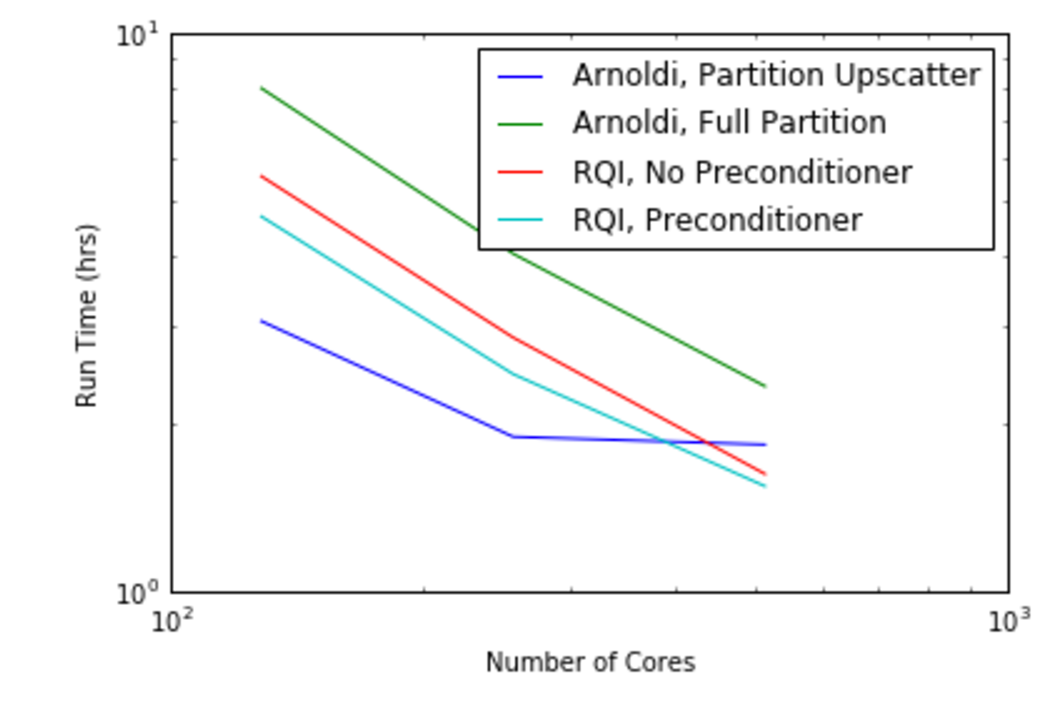
\includegraphics[scale=.5]{Remus_Scaling}
\centering
\end{figure}

 On the cluster, the study was performed with 128, 256, and 512 cores and 1, 2, and 4 energy sets. It showed favorable scaling on behalf of the RQI methods, whereas Arnoldi with upscatter partitioning shows poor scaling performance after two energy sets. 

\begin{figure}
\label{fig:titan}
\caption{Energy set scaling study on Titan}
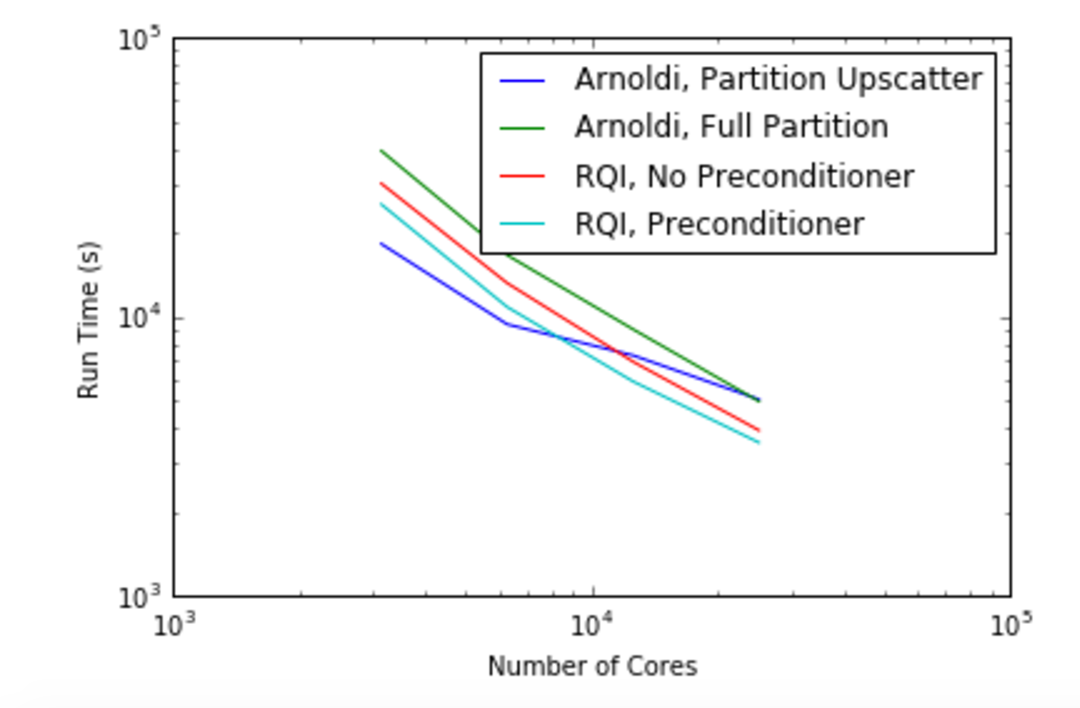
\includegraphics[scale=.5]{Titan_Scaling}
\centering
\end{figure}

On Titan, the intial problem was run with 3,136 cores (56 x-blocks, 56 y-blocks, and 1 set). We then scaled up to 2, 4, and 8 sets and 6,272, 12,544, and 25,088 cores, respectively. The upscatter and k-tolerances were set to $1 \times 10^{-5}$. A parallel-efficiency modeling tool developed at Oak Ridge was used to choose the optimal z-blocks for each method, which in the case of RQI with MGE preconditioning was determined to be 22. For the other three methods, 11 z-blocks were determined to be optimal. Based on previous studies \cite{Slaybaugh2015}, a weight of 1 was chosen with 3 v-cycles and 2 relaxations. 
%---------------------------------------------------------------------------%%

\section{Conclusions}
\label{sec:conclusions}
The goal of this research was to accelerate transport calculations with methods that can take full advantage of modern leadership-class comuputers, facilitating the design of better nuclear systems. Three complimentary methods were implemented that accomplish this goal to varying degrees. 

At the outset of this work, Denovo could be decomposed in five of the six dimensions of phase space over which the steady-state transport equation is solved in a way that restricted it to about 20,000 cores for a problem with 500 million cells. The original suite of solvers included Gauss Seidel as the multigroup solver and power iteration wrapped around GS as the eigenvalue solver. These solvers have some significant limitations in many cases of interest. 

The new multigroup Krylov solver converges more quickly than GS and enables energy decomposition such that Denovo can scale to hundreds of thousands of cores. The new multigrid-in-energy preconditioner reduces iteration count for many problem types and takes advantage of the new energy decomposition such that it can scale very efficiently. These two tools are useful on their own, but together they allow the Rayleigh Quotient Iteration eigenvalue solver to work.

The real motivation of this work was to add RQI, which should converge in fewer iterations that power iteration for large and challenging problems. RQI creates shifted systems that would not be tractable without the MG Krylov solver. It also creates ill-conditioned matrices that cannot converge without the multigrid-in-energy preconditioner. Using these methods, RQI converged in fewer iterations and in less time than preconditioned PI for a full-facility PWR on 200,000 cores. 

The methods added in this research accelerated Denovo in multiple ways. This acceleration helps enable the solution of today’s “grand challenge” problems. It is hoped that improved methods will lead to improved reactor designs and systems, and that the frontier of computational challenges will be moved forward.

%---
Rayleigh Quotient Iteration is an old method that is an adaptation of shifted inverse iteration. Because the RQ provides an optimal shift, it is expected that using RQI in Denovo will converge in fewer iterations than power iteration for loosely coupled problems, provided that the eigenvector is converged. 

Further, this solver is wrapped around the new MG Krylov solver. It has been shown that the energy decomposition improves solution time and scales well \cite{Slaybaugh2011}. It is therefore reasonable to expect that when RQI converges, decomposing the entire matrix in energy for eigenvalue calculations will work and provide the same kind of scaling improvement.

RQI has not been applied to the transport equation before. This is likely because it takes $O(n^{3})$ operations for full dense matrices, and without parallelization in energy it could be prohibitively expensive \cite{Stewart2001}. In the past, adding a shift to make the scattering matrix energy-block dense was difficult to handle. The system would have been solved with Gauss Seidel, which would have been restrictively slow. The multigroup Krylov algorithm has enabled energy parallelization and made the calculation of the eigenvector tractable. 

Computers that facilitate enough parallelization to decompose in energy and have enough memory to store Krylov subspaces for the full transport equation make combining RQI and MG Krylov possible. The resulting convergence of the eigenvalue should be faster than PI for at least some problems. The energy decomposition will allow eigenvalue calculations to overcome the limitations of scaling in space and angle alone such that the code can be scaled to many more cores. These ideas have never before been used together in this way.  


%%---------------------------------------------------------------------------%%

\section{Acknowledgements}

This research used resources of the Oak Ridge Leadership Computing Facility at the Oak Ridge National Laboratory, which is supported by the Office of Science of the U.S. Department of Energy under Contract No. DE-AC05-00OR22725. Additional thanks to the Rickover Fellowship Program in Nuclear Engineering sponsored by Naval Reactors Division of the U.S. Department of Energy. This fellowship sponsored the work from which this work is derived. 

%%---------------------------------------------------------------------------%%

\newpage
\appendix

\section{Angular Flux Moments}
\label{sec:angular-flux-moments}

Appendix

%%---------------------------------------------------------------------------%%
%% BIBLIOGRAPHY
%%---------------------------------------------------------------------------%%

\newpage

\singlespacing

\bibliographystyle{model1-num-names}
\bibliography{RQI_MGE}

%%---------------------------------------------------------------------------%%
%% TABLES
%%---------------------------------------------------------------------------%%

\clearpage

\begin{table}[p]
  \caption{
    Comparison of results for the adjoint neutron porosity tool
    problem. For these problems, the adjoint source is place in the
    far detector.  All timing results are normalized to the
    unaccelerated Gauss-Seidel iteration time.
  }
  \label{tab:adjoint-porosity-tool}
  \begin{center}
    \begin{tabular}{lcll}\hline\hline
      Method & Acceleration $S_N$ order & GS iterations & Time \\\hline
      %%
      GS & - & 53 & 1.0   \\
      TTG & 8 & 7 & 0.172 \\
      TTG & 2 & 7 & 0.159 \\
      \hline\hline
    \end{tabular}
  \end{center}
\end{table}

%%---------------------------------------------------------------------------%%

\clearpage

\begin{table}[p]
  \caption{
    Results from the neutron porosity tool problem using MTTG.  All
    timing results are normalized to the unaccelerated Gauss-Seidel
    iteration time.
  }
  \label{tab:MTTG-porosity-tool}
  \begin{center}
    \begin{tabular}{llllll}\hline\hline
      Method & Acceleration $S_N$  & GS Iterations & Within-group
      & Acceleration & Time \\
      & order & & sweeps & sweeps &  \\\hline
      %%
      GS   & - & 175 & 16294 & 0    & 1.0   \\
      TTG  & 8 & 15  & 1398  & 547  & 0.113 \\
      TTG  & 2 & 13  & 1212  & 459  & 0.086 \\
      MTTG & 2 & 47  & 611   & 1329 & 0.050 \\
      \hline\hline
    \end{tabular}
  \end{center}
\end{table}

%%---------------------------------------------------------------------------%%
%% FIGURES
%%---------------------------------------------------------------------------%%

\clearpage

\begin{figure}[p]
  \begin{center}
    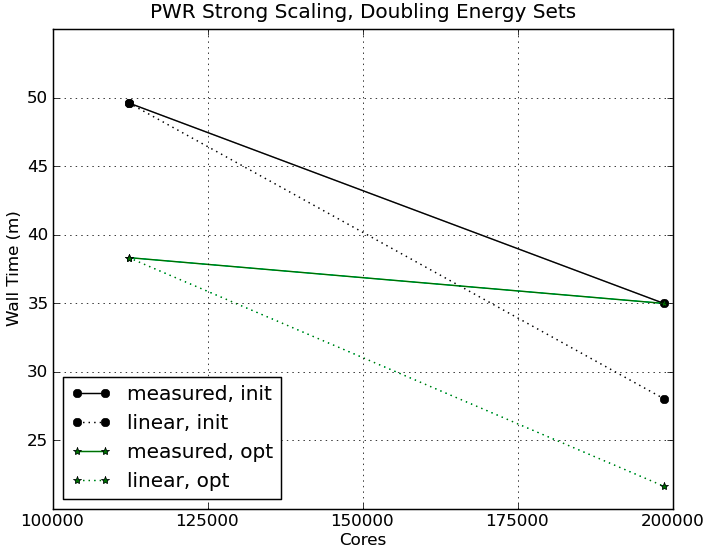
\includegraphics[width=6in,clip]{PWRstrongScaling}
  \end{center}
  \caption{Example1}
  \label{fig:example1}
\end{figure}

%%---------------------------------------------------------------------------%%

\clearpage

\begin{figure}[p]
  \begin{center}
    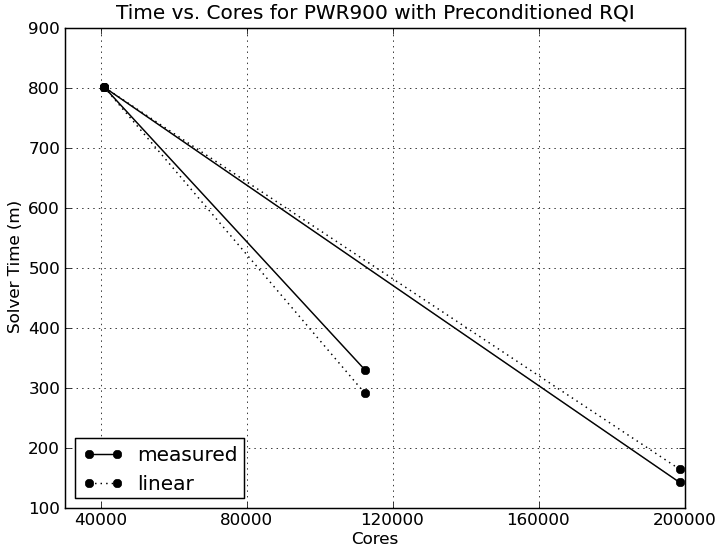
\includegraphics[width=6in,clip]{PWRPrecondRQI}
  \end{center}
  \caption{Example}
  \label{fig:example2}
\end{figure}

%%---------------------------------------------------------------------------%%

\clearpage

\singlespacing
\begin{center}

  {\Large \bf Title}
  
  \vspace{0.3in}
  
  {\large R.N. Slaybaugh\footnote{Corresponding author.  Telephone: +1
      570 850 3385.  E-mail: rns37@pitt.edu.}\\
    Department of Mechanical Engineering and Material Science\\
    University of Pittsburgh\\
    605 Benedum Hall, 3700 O'Hara Street\\
    Pittsburgh, PA 15261, USA\\\vspace{1\baselineskip}
    T.M. Evans, G.G. Davidson\\
    Radiation Transport and Criticality Group\\ 
    Oak Ridge National Laboratory\\ 
    P.O. Box 2008\\
    Oak Ridge, TN 37831-6170, USA\\\vspace{1\baselineskip}
    P.P.H. Wilson\\
    Department of Nuclear Engineering and Engineering Physics\\
    University of Wisconsin -- Madison\\
    419 ERB, 1500 Engineering Drive\\
    Madison, WI 52706, USA\\}
  
  \addtocounter{page}{-1}

  \vspace{2.0in}
  \renewcommand{\thetable}{\arabic{table}}
  \thepage\ Pages --- \thetable\ Tables --- \thefigure\ Figures \\

  \setcounter{page}{1}

\end{center}

%%---------------------------------------------------------------------------%%

\end{document}

%%---------------------------------------------------------------------------%%
%% end of paper.tex
%%---------------------------------------------------------------------------%%
